\documentclass[8pt,aspectratio=169]{beamer}
\usepackage{minted}

% There are many different themes available for Beamer. A comprehensive
% list with examples is given here:
% http://deic.uab.es/~iblanes/beamer_gallery/index_by_theme.html
% You can uncomment the themes below if you would like to use a different
% one:
%\usetheme{AnnArbor}
%\usetheme{Antibes}
%\usetheme{Bergen}
%\usetheme{Berkeley}
%\usetheme{Berlin}
%\usetheme{Boadilla}
%\usetheme{boxes}
%\usetheme{CambridgeUS}
%\usetheme{Copenhagen}
%\usetheme{Darmstadt}
%\usetheme{default}
%\usetheme{Frankfurt}
%\usetheme{Goettingen}
%\usetheme{Hannover}
%\usetheme{Ilmenau}
%\usetheme{JuanLesPins}
%\usetheme{Luebeck}
\usetheme{Madrid}
%\usetheme{Malmoe}
%\usetheme{Marburg}
%\usetheme{Montpellier}
%\usetheme{PaloAlto}
%\usetheme{Pittsburgh}
%\usetheme{Rochester}
%\usetheme{Singapore}
%\usetheme{Szeged}
%\usetheme{Warsaw}

\title{Teaching a Computer to Diagnose Cancer}
\subtitle{An Introduction to Machine Learning}

\author{Glenn R. Fisher}
% - Give the names in the same order as the appear in the paper.
% - Use the \inst{?} command only if the authors have different
%   affiliation.

\institute[IBM Mobile Innovation Lab] % (optional, but mostly needed)

% \date{Conference Name, 2013}
% - Either use conference name or its abbreviation.
% - Not really informative to the audience, more for people (including
%   yourself) who are reading the slides online

\subject{Machine Learning}
% This is only inserted into the PDF information catalog. Can be left
% out. 

% If you have a file called "organization-logo-filename.xxx", where xxx
% is a graphic format that can be processed by latex or pdflatex,
% resp., then you can add a logo as follows:

\pgfdeclareimage[height=0.5cm]{organization-logo}{figures/MIL_Logo_BW}
\logo{\pgfuseimage{organization-logo}}

% Delete this, if you do not want the table of contents to pop up at
% the beginning of each subsection:
\AtBeginSubsection[]
{
  \begin{frame}<beamer>{Outline}
    \tableofcontents[currentsection,currentsubsection]
  \end{frame}
}

% Let's get started
\begin{document}

\begin{frame}
  \titlepage
\end{frame}

% \begin{frame}{Outline}
%   \tableofcontents[hideallsubsections]
%   % You might wish to add the option [pausesections]
% \end{frame}

%%%%%%%%%%%%%%%%%%%%%%%%%%%%%%%%%%%%%%%%%%%%%%%%%%%%%%%%%%%%%%%%%%%%%%%%%%%%%%%%
% Section - What is Machine Learning?
%%%%%%%%%%%%%%%%%%%%%%%%%%%%%%%%%%%%%%%%%%%%%%%%%%%%%%%%%%%%%%%%%%%%%%%%%%%%%%%%

\section{What is Machine Learning?}

%%%%%%%%%%
% Slide
%%%%%%%%%%

\begin{frame}{What is Machine Learning?}

\pause
Machine learning uses computer programs to learn relationships in data.
\newline

\begin{itemize}
\item \pause
  \textbf{Supervised Learning}:
    \begin{itemize}
    \item \pause Data is organized into input-output pairs.
    \item \pause The goal is to learn the relationship between inputs and outputs.
    \end{itemize}
\vspace{3mm}
\item \pause
  \textbf{Unsupervised Learning}:
    \begin{itemize}
    \item \pause Data is \textit{not} organized into input-output pairs.
    \item \pause The goal is to learn the relationship between data points.
    \item \pause This is also known as data mining, clustering, etc.
    \end{itemize}
\end{itemize}

\end{frame}

%%%%%%%%%%%%%%%%%%%%%%%%%%%%%%%%%%%%%%%%%%%%%%%%%%%%%%%%%%%%%%%%%%%%%%%%%%%%%%%%
% Section - Supervised Learning
%%%%%%%%%%%%%%%%%%%%%%%%%%%%%%%%%%%%%%%%%%%%%%%%%%%%%%%%%%%%%%%%%%%%%%%%%%%%%%%%

\section{Supervised Learning}

%%%%%%%%%%
% Slide
%%%%%%%%%%

\begin{frame}{Supervised Learning}

\textbf{Supervised Learning:}
\newline

\begin{itemize}
\item \pause
  Data: $(\vec{x_1}, y_1), (\vec{x_2}, y_2), ..., (\vec{x_n}, y_n)$
\item \pause
  Assumption: The data was generated by some function, $f(\vec{x_i}) = y_i$
\item \pause
  Goal: Learn the function, $f(\vec{x_i})$
\end{itemize}

\vspace{-3.5mm}

\pause
\begin{columns}[T] % align columns
\begin{column}{.2\textwidth}
\begin{center}
  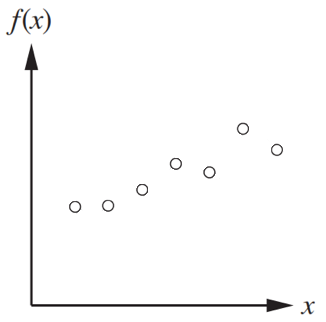
\includegraphics[scale=0.65]{figures/supervised-learn-f-1}
\end{center}
\end{column}

\pause
\begin{column}{.2\textwidth}
\begin{center}
  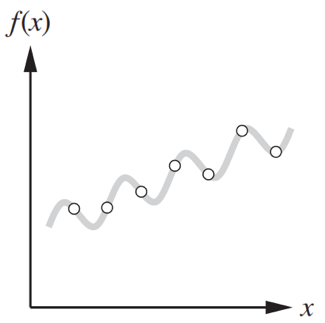
\includegraphics[scale=0.65]{figures/supervised-learn-f-2}
\end{center}
\end{column}

\pause
\begin{column}{.2\textwidth}
\begin{center}
  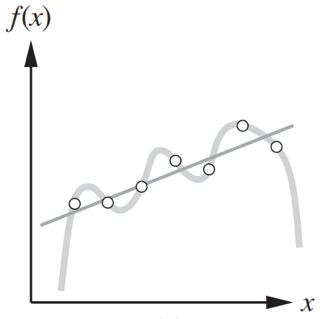
\includegraphics[scale=0.65]{figures/supervised-learn-f-3}
\end{center}
\end{column}
\end{columns}

\end{frame}

%%%%%%%%%%
% Slide
%%%%%%%%%%

\begin{frame}{Types of Supervised Learning}

\begin{columns}[T] % align columns
\begin{column}{.48\textwidth}
\pause
\begin{center}
  Regression: Numerical Outputs
  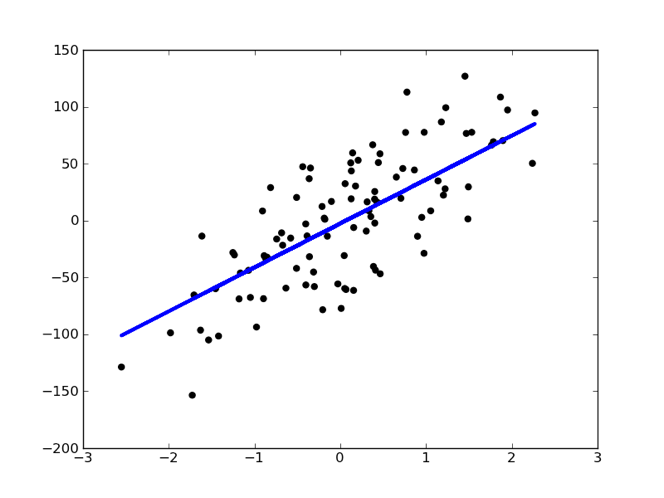
\includegraphics[scale=0.6]{figures/supervised-regression}
\end{center}
\end{column}

\begin{column}{.48\textwidth}
\pause
\begin{center}
  Classification: Categorical Outputs
  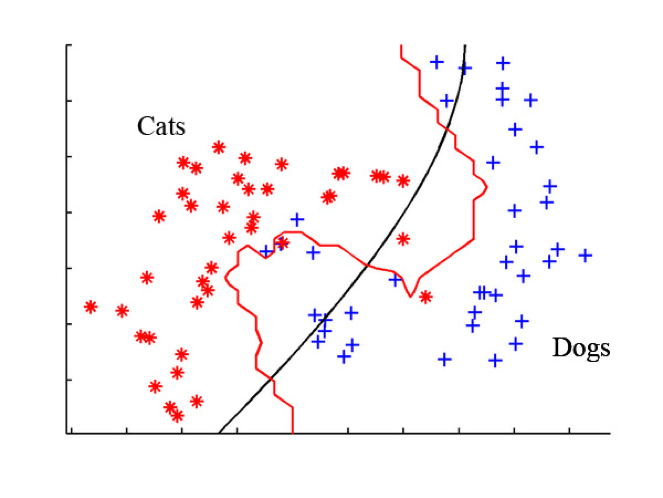
\includegraphics[scale=0.63]{figures/supervised-classification}
\end{center}
\end{column}
\end{columns}

\end{frame}

%%%%%%%%%%
% Slide
%%%%%%%%%%

\begin{frame}{Supervised Learning Examples}

\pause
\begin{columns}[T]
\begin{column}{.33\textwidth}
\begin{center}
  \frame{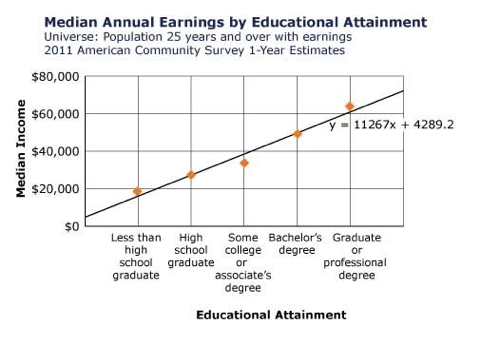
\includegraphics[scale=0.63]{figures/example-income.png}}
  \vspace{-1mm}

  Input: Years of Education\\
  Output: Annual Income\\
  Application: Predict Income
\end{center}
\end{column}

\pause
\begin{column}{.33\textwidth}
\begin{center}
  \frame{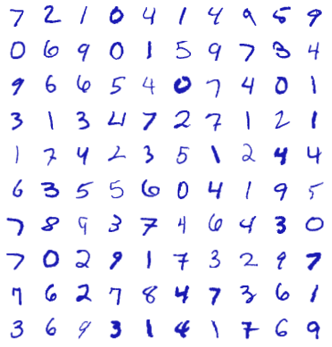
\includegraphics[scale=0.63]{figures/example-handwriting.png}}
  \vspace{2mm}

  Input: Pictures of Written Digits\\
  Output: Intended Digit\\
  Application: Zip-Code Mail Sorting
\end{center}
\end{column}

\pause
\begin{column}{.33\textwidth}
\begin{center}
  \frame{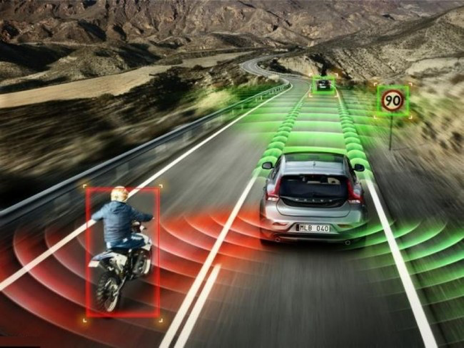
\includegraphics[scale=0.63]{figures/example-cars.png}}
  \vspace{2mm}

  Input: Environment Sensors\\
  Output: Driving Instructions\\
  Application: Self-Driving Cars
\end{center}
\end{column}
\end{columns}

\end{frame}

% %%%%%%%%%%%%%%%%%%%%%%%%%%%%%%%%%%%%%%%%%%%%%%%%%%%%%%%%%%%%%%%%%%%%%%%%%%%%%%%%
% % Section - Unsupervised Learning
% %%%%%%%%%%%%%%%%%%%%%%%%%%%%%%%%%%%%%%%%%%%%%%%%%%%%%%%%%%%%%%%%%%%%%%%%%%%%%%%%

% \section{Unsupervised Learning}

% %%%%%%%%%%
% % Slide
% %%%%%%%%%%

% \begin{frame}{Unsupervised Learning}

% \pause
% \textbf{Unsupervised Learning}
% \newline

% \begin{itemize}
% \item \pause
%   Data: $\vec{x_1}, \vec{x_2}, ..., \vec{x_n}$
% \item \pause
%   Assumption: There are hidden patterns in the data
% \item \pause
%   Goal: Identify the hidden patterns
% \end{itemize}

% \vspace{2mm}

% \pause
% \begin{center}
%   \raisebox{-.5\height}{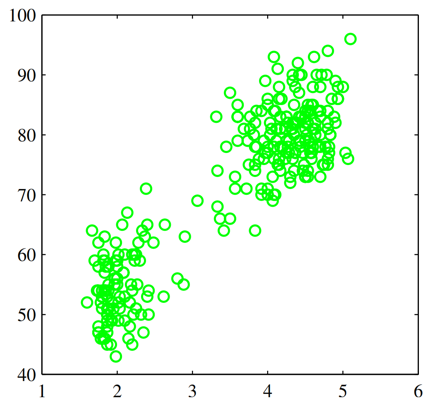
\includegraphics[scale=0.5]{figures/unsupervised-clustering-before}}
%   \raisebox{-.5\height}{\scalebox{4}{$\Rightarrow$}}
%   \raisebox{-.5\height}{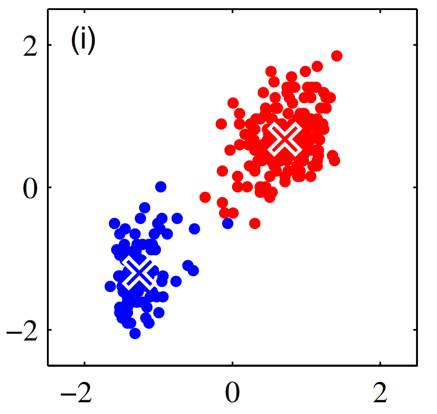
\includegraphics[scale=0.5]{figures/unsupervised-clustering-after}}
%   \vspace{3mm}

%   Clustering algorithm applied to Old Faithful geyser eruption data.\\
%   (Horizontal Axis: Eruption Duration; Vertical Axis: Time to Next Eruption)
% \end{center}

% \end{frame}

%%%%%%%%%%%%%%%%%%%%%%%%%%%%%%%%%%%%%%%%%%%%%%%%%%%%%%%%%%%%%%%%%%%%%%%%%%%%%%%%
% Section - Identifying Cancer Cells
%%%%%%%%%%%%%%%%%%%%%%%%%%%%%%%%%%%%%%%%%%%%%%%%%%%%%%%%%%%%%%%%%%%%%%%%%%%%%%%%

\section{Identifying Cancer Cells}

%%%%%%%%%%
% Slide
%%%%%%%%%%

\begin{frame}{Identifying Cancer Cells}

\begin{center}
  \pause
  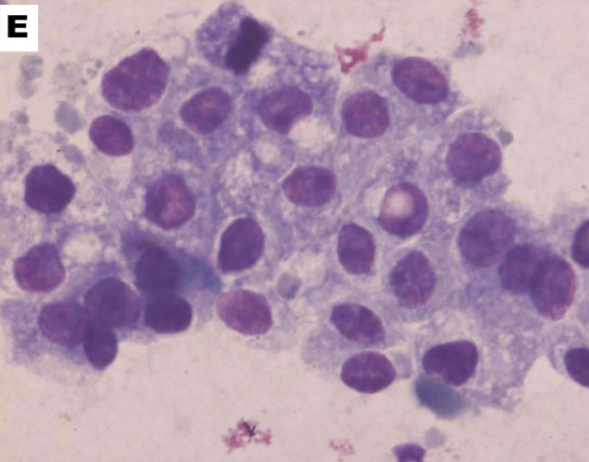
\includegraphics[scale=0.5]{figures/cancer-cells}
  \vspace{5mm}

  \pause
  \LARGE Are these cancer cells?\\
  \normalsize
  1. Yes, they are malignant.\\
  2. No, they are benign.
\end{center}

\end{frame}

%%%%%%%%%%
% Slide
%%%%%%%%%%

\begin{frame}{Identifying Cancer Cells: Problem Formulation}

\begin{itemize}
\pause \item What are the inputs? \pause $\Rightarrow$ The shape of each cell.
\pause \item What are the outputs? \pause $\Rightarrow$ A diagnosis (malignant or benign).
\pause \item What are our assumptions? \pause $\Rightarrow$ There is a relationship between cell shape and cancer.
\pause \item What is our goal? \pause $\Rightarrow$ Learn the relationship between cell shape and cancer.
\pause \item What data will we use to solve our goal? \pause $\Rightarrow$ Wisconsin Diagnostic Breast Cancer (WDBC).
\end{itemize}

\vspace{2mm}

\pause
\begin{center}
 \begin{tabular}{|c c c|} 
 \hline
 Diagnosis & Radius & Texture \\ [0.25ex] 
 \hline
 Malignant & 16.08 & 21.82 \\
 Malignant & 25.28 & 25.59 \\
 Benign    & 14.48 & 21.82 \\
 ...       & ...   & ...   \\
 Malignant & 20.92 & 34.69 \\ [1ex] \hline
\end{tabular}
\end{center}

\end{frame}

%%%%%%%%%%
% Slide
%%%%%%%%%%

\begin{frame}{Identifying Cancer Cells: Data Exploration}

\pause
\begin{center}
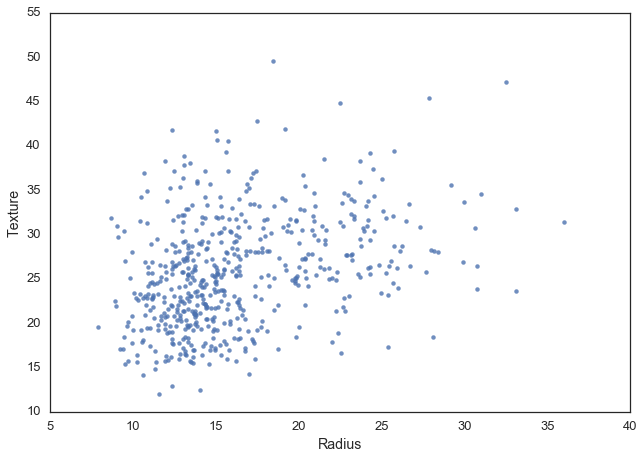
\includegraphics[scale=0.40]{figures/cancer-scatter-plot}
\end{center}

\end{frame}

%%%%%%%%%%
% Slide
%%%%%%%%%%

\begin{frame}{Identifying Cancer Cells: Data Exploration}

\begin{center}
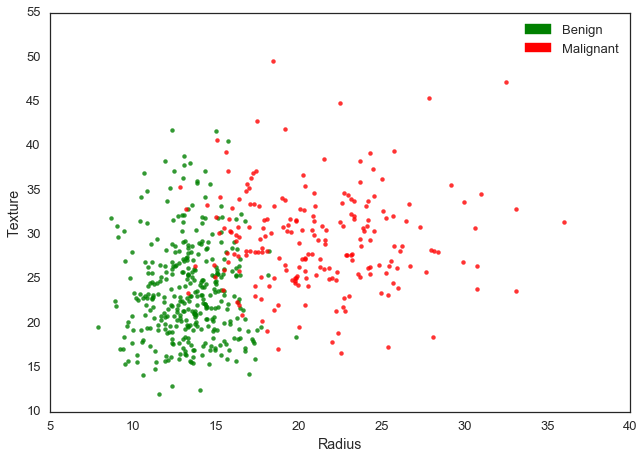
\includegraphics[scale=0.40]{figures/cancer-scatter-plot-by-class}
\end{center}

\end{frame}

%%%%%%%%%%
% Slide
%%%%%%%%%%

\begin{frame}{Identifying Cancer Cells: Data Exploration}

\begin{center}
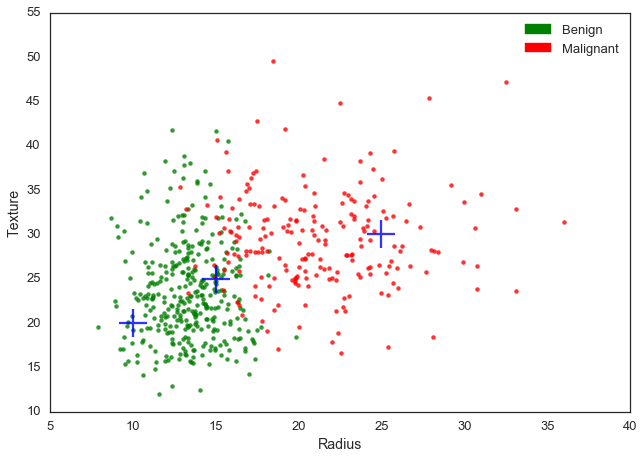
\includegraphics[scale=0.40]{figures/cancer-scatter-plot-examples}
\end{center}

\end{frame}

%%%%%%%%%%
% Slide
%%%%%%%%%%

\begin{frame}{Identifying Cancer Cells: k-Nearest Neighbors Algorithm}

\pause
k-Nearest Neighbors Algorithm: Classify an observation according to the class of its neighbors.

\begin{columns}[T]
\begin{column}{.48\textwidth}
\begin{center}
\pause
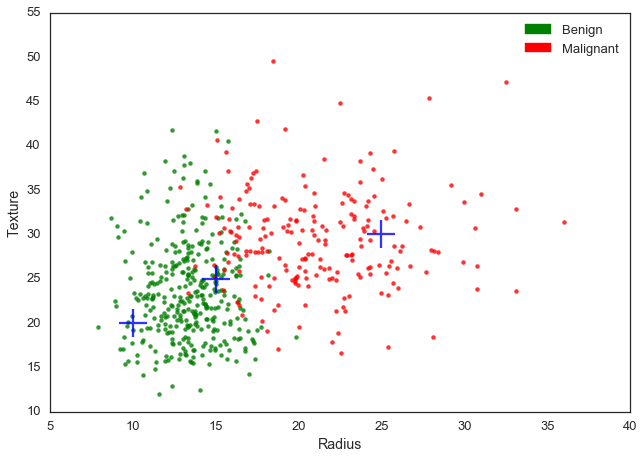
\includegraphics[scale=0.30]{figures/cancer-scatter-plot-examples}
\end{center}
\end{column}

\begin{column}{.48\textwidth}
\vspace{5mm}
\pause
How It Works:

\begin{enumerate}
\pause \item Consider observations as points in space.
\pause \item Given a new observation to classify, find its k nearest neighbors.
\pause \item Among these neighbors, find the most common class.
\pause \item Use that class to classify the new observation.
\end{enumerate}
\end{column}
\end{columns}

\end{frame}

%%%%%%%%%%
% Slide
%%%%%%%%%%

\begin{frame}[fragile]{Identifying Cancer Cells: Model Training}

\pause
1. Load the dataset.

\pause
\begin{minted}{python}
    columns_to_features = { 1: "Diagnosis",
                           22: "Radius",
                           23: "Texture"}
\end{minted}
\pause
\begin{minted}{python}
    features_to_keep = columns_to_features.values()
\end{minted}
\pause
\begin{minted}{python}
    wdbc = pd.read_csv("wdbc.data", header = None) \
             .rename(columns = columns_to_features) \
             .filter(features_to_keep, axis = 1) \
             .replace("M", "Malignant") \
             .replace("B", "Benign")
\end{minted}

\pause
2. Split dataset into separate training and test sets.

\pause
\begin{minted}{python}
    x_full = wdbc.drop("Diagnosis", axis = 1)
    y_full = wdbc["Diagnosis"]
    x_train, x_test, y_train, y_test = sklearn.cross_validation.train_test_split(
        x_full, y_full, test_size = 0.3, random_state = 3)
\end{minted}

\pause
3. Train a k-nearest neighbors classifier.

\pause
\begin{minted}{python}
    model = sklearn.neighbors.KNeighborsClassifier().fit(x_train, y_train)
\end{minted}

\end{frame}

%%%%%%%%%%
% Slide
%%%%%%%%%%

\begin{frame}[fragile]{Identifying Cancer Cells: Model Evaluation}

\pause
We want to know how well our model generalizes. How accurately can it predict a diagnosis?

\vspace{3mm}
\pause
To answer this question, we will:

\begin{enumerate}
\pause \item Use the trained model to predict a diagnosis for each observation in the test set.
\pause \item Compare each prediction with that observation's actual diagnosis.
\pause \item Compute model accuracy as the fraction of correct predictions.
\end{enumerate}

\vspace{3mm}
\pause
This is a straightforward computation in Python:

\pause
\begin{minted}{python}
    predictions = model.predict(x_test)
\end{minted}
\pause
\begin{minted}{python}
    sklearn.metrics.accuracy_score(predictions, y_test)
\end{minted}

\vspace{3mm}
\pause
We find that our simple k-nearest neighbors classifier has 95\% accuracy!

\vspace{3mm}
\pause
\textbf{We just trained a computer to correctly diagnose breast cancer cells 95\% of the time.}

\end{frame}

%%%%%%%%%%
% Slide
%%%%%%%%%%

\begin{frame}[fragile]{Identifying Cancer Cells: The Program}

\pause
\begin{minted}{python}
# load dataset
columns_to_features = { 1: "Diagnosis",
                       22: "Radius",
                       23: "Texture"}
features_to_keep = columns_to_features.values()
wdbc = pd.read_csv("wdbc.data", header = None) \
         .rename(columns = columns_to_features) \
         .filter(features_to_keep, axis = 1) \
         .replace("M", "Malignant") \
         .replace("B", "Benign")
\end{minted}

\pause
\begin{minted}{python}
# split dataset into training and test sets
x_full = wdbc.drop("Diagnosis", axis = 1)
y_full = wdbc["Diagnosis"]
x_train, x_test, y_train, y_test = sklearn.cross_validation.train_test_split(
    x_full, y_full, test_size = 0.3, random_state = 3)
\end{minted}

\pause
\begin{minted}{python}
# train a k-nearest neighbors model
model = sklearn.neighbors.KNeighborsClassifier().fit(x_train, y_train)
\end{minted}

\pause
\begin{minted}{python}
# evaluate the model's accuracy
predictions = model.predict(x_test)
sklearn.metrics.accuracy_score(predictions, y_test)
\end{minted}

\end{frame}

%%%%%%%%%%%%%%%%%%%%%%%%%%%%%%%%%%%%%%%%%%%%%%%%%%%%%%%%%%%%%%%%%%%%%%%%%%%%%%%%
% Section - Recap
%%%%%%%%%%%%%%%%%%%%%%%%%%%%%%%%%%%%%%%%%%%%%%%%%%%%%%%%%%%%%%%%%%%%%%%%%%%%%%%%

\section{Recap}

%%%%%%%%%%
% Slide
%%%%%%%%%%

\begin{frame}{Recap}

Let's review some of the big ideas:

\begin{itemize}
\pause \item Machine Learning: Use computer programs to learn relationships in data.
\pause \item Supervised Learning: Learn relationships between inputs and outputs.
	\begin{itemize}
	\pause \item Regression: Numerical outputs.
	\pause \item Classification: Categorical outputs.
	\end{itemize}
\pause \item Unsupervised Learning: Learn relationships between data points.
\pause \item k-Nearest Neighbors Algorithm: Classify an observation according to its neighbors.
\pause \item Diagnosing Cancer: We trained a model to diagnose cancer with 95\% accuracy.
\end{itemize}

\end{frame}

\end{document}

%%%%%%%%%%%%%%%%%%%%%%%%%%%%%%%%%%%%%%%%%%%%%%%%%%%%%%%%%%%%%%%%%%%%%%%%%%%%%%%%
% Tips and tricks from template
%%%%%%%%%%%%%%%%%%%%%%%%%%%%%%%%%%%%%%%%%%%%%%%%%%%%%%%%%%%%%%%%%%%%%%%%%%%%%%%%

% % You can reveal the parts of a slide one at a time
% % with the \pause command:
% \begin{frame}{Second Slide Title}
%   \begin{itemize}
%   \item {
%     First item.
%     \pause % The slide will pause after showing the first item
%   }
%   \item {   
%     Second item.
%   }
%   % You can also specify when the content should appear
%   % by using <n->:
%   \item<3-> {
%     Third item.
%   }
%   \item<4-> {
%     Fourth item.
%   }
%   % or you can use the \uncover command to reveal general
%   % content (not just \items):
%   \item<5-> {
%     Fifth item. \uncover<6->{Extra text in the fifth item.}
%   }
%   \end{itemize}
% \end{frame}

% \begin{frame}{Blocks}
% \begin{block}{Block Title}
% You can also highlight sections of your presentation in a block, with it's own title
% \end{block}
% \begin{theorem}
% There are separate environments for theorems, examples, definitions and proofs.
% \end{theorem}
% \begin{example}
% Here is an example of an example block.
% \end{example}
% \end{frame}

% % Placing a * after \section means it will not show in the
% % outline or table of contents.
% \section*{Summary}

% \begin{frame}{Summary}
%   \begin{itemize}
%   \item
%     The \alert{first main message} of your talk in one or two lines.
%   \item
%     The \alert{second main message} of your talk in one or two lines.
%   \item
%     Perhaps a \alert{third message}, but not more than that.
%   \end{itemize}
  
%   \begin{itemize}
%   \item
%     Outlook
%     \begin{itemize}
%     \item
%       Something you haven't solved.
%     \item
%       Something else you haven't solved.
%     \end{itemize}
%   \end{itemize}
% \end{frame}

% % All of the following is optional and typically not needed. 
% \appendix
% \section<presentation>*{\appendixname}
% \subsection<presentation>*{For Further Reading}

% \begin{frame}[allowframebreaks]
%   \frametitle<presentation>{For Further Reading}
    
%   \begin{thebibliography}{10}
    
%   \beamertemplatebookbibitems
%   % Start with overview books.

%   \bibitem{Author1990}
%     A.~Author.
%     \newblock {\em Handbook of Everything}.
%     \newblock Some Press, 1990.
 
    
%   \beamertemplatearticlebibitems
%   % Followed by interesting articles. Keep the list short. 

%   \bibitem{Someone2000}
%     S.~Someone.
%     \newblock On this and that.
%     \newblock {\em Journal of This and That}, 2(1):50--100,
%     2000.
%   \end{thebibliography}
% \end{frame}
